\chapter{A Simple Adaptive-Trajectory Method}
\label{ch:simple_method}

The preceding chapters develop an evidence-management view of MP-VRDU and identify where failures arise within representation, selection, and reasoning. This chapter translates those findings into a deliberately simple working system and evaluates whether they remain useful when combined.

\section{Introduction}
\label{sec:simple_method_intro}

We introduce a simple adaptive evidence-management pipeline designed directly from the findings of Chapters~\ref{ch:survey} and~\ref{ch:empirical}. Rather than introducing a specialised document backbone or complex orchestration framework, the method combines broad evidence acquisition, selective evidence presentation, and structured reasoning within an adaptive trajectory. The aim is to test whether these principles are sufficient to produce a competitive MP-VRDU system while retaining a transparent and configurable design.

\textbf{Our contributions are as follows:} \textbf{(1)} We introduce a simple adaptive evidence-management pipeline that achieves performance competitive with leading MP-VRDU systems using the same backbone. \textbf{(2)} We provide a system-level validation of the evidence-management perspective and empirical attribution findings by translating them into concrete choices over representation, selection, and reasoning. \textbf{(3)} We characterise the resulting deployment trade-offs through configurable evidence-coverage and trajectory parameters, together with measurements of token usage, latency, memory use, and trajectory length.

\section{Methodology}
\label{sec:simple_adaptive_method}

We combines high-fidelity multimodal representation, broad evidence acquisition, selective evidence presentation, and structured reasoning. Its design follows the three failure loci identified in the attribution study. For \textbf{representation}, pages are read through complementary textual and visual channels so that evidence lost or difficult to access through one remains available through the other. For \textbf{selection}, the system favours broad evidence acquisition because additional pages can either disrupt or repair an answer depending on the context they contribute; evidence gathering is therefore separated from deciding which pages should be exposed in full to the final reasoner. For \textbf{reasoning}, the final answer is produced with explicit intermediate reasoning, premise checking, and abstention so that the gathered evidence is both integrated and checked for sufficiency. The resulting pipeline uses three specialised roles implemented by the same underlying vision-language model:

\begin{enumerate}
    \item The \texttt{reader} traverses pages in retrieval-ranked order, records answer-relevant evidence from each page, marks pages likely to contain answer-bearing information, and decides when sufficient evidence has been collected to attempt an answer.
    \item The \texttt{synthesizer} receives the accumulated evidence in document order. Pages marked as answer-bearing are supplied in full through their textual and visual representations, while other useful pages remain available through the compact records produced by the \texttt{reader}. It then reasons over the assembled evidence and produces a candidate answer.
    \item The \texttt{arbiter} receives the accumulated evidence and candidate answer and decides whether the current evidence is sufficient to terminate the trajectory or whether control should return to the \texttt{reader} for further evidence acquisition. It cannot replace the answer itself.
\end{enumerate}

\begin{figure}[ht]
    \centering
    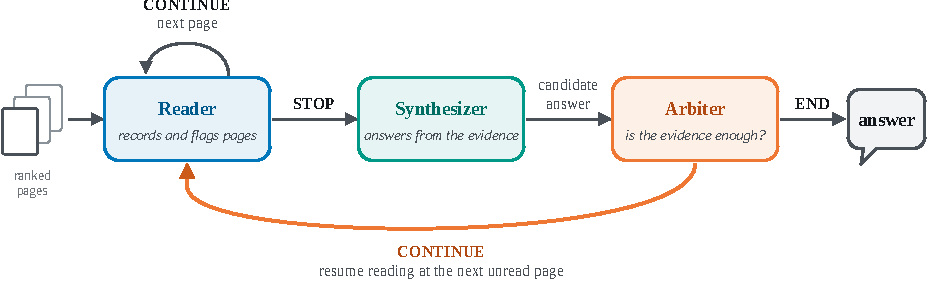
\includegraphics[width=0.9\columnwidth]{method/simple_method.pdf}
    \caption{Architecture of our simple method.}
    \label{fig:simple_method_architecture}
\end{figure}

The three roles form an adaptive evidence-processing loop. When the \texttt{reader} proposes \texttt{STOP}, the \texttt{synthesizer} receives the retained records and full representations of pages marked as answer-bearing, with the highest-ranked read pages used as fallback when none are marked. It then reasons over the evidence, checks question premises, and must identify the missing fact before returning \emph{Not answerable}. The \texttt{arbiter} either accepts the answer or resumes reading from the next unread page. Full prompts and implementation details are provided in Appendix~\ref{app:simple_method_details}.

\paragraph{Configuration.} We instantiate all three roles with a shared 4-bit NF4 \texttt{Qwen3-VL-8B-Instruct} model using greedy decoding. Document pages are ranked once per question using ColQwen3.5 and visited in that order. The \texttt{reader} processes pages using the full \textbf{TLV} representation, combining Unlimited-OCR text with the high-resolution visual preset. During synthesis, every page marked as answer-bearing is reintroduced through its Unlimited-OCR text and page image at medium resolution, while unflagged pages contribute only their retained records. This preserves the redundant text and vision channels identified as beneficial in Chapter~\ref{ch:empirical} while limiting the amount of full multimodal context presented.

\paragraph{Deployment parameters.} Five parameters control the amount and depth of evidence acquisition. \(B\) sets the maximum number of pages that may be read, \(p\) controls the number of pages processed per \texttt{reader} turn, \(k\) sets the minimum initial reading depth before stopping is allowed, \(m\) sets the minimum additional reading after the \texttt{arbiter} reopens a trajectory, and \(C\) bounds the number of synthesis attempts. These parameters allow the same pipeline to scale across deployment settings: larger budgets increase evidence coverage and trajectory depth, while smaller values reduce latency, token use, and memory pressure.

\section{Experiments}
\label{sec:simple_method_experiments}

\paragraph{Setup and comparison.} We reuse the experimental infrastructure of Chapter~\ref{ch:empirical}, including, document preprocessing, evaluation, and the Qwen3-VL model family. The deployment configuration is chosen specifically to run on a single NVIDIA V100 16\,GB GPU, using 4-bit NF4 Qwen3-VL-8B-Instruct with FP16 compute and greedy decoding, with \(B=25\), \(p=1\), \(k=6\), \(m=3\), and \(C=3\). We report answer accuracy overall, by evidence source, and on unanswerable questions. We compare against M3DocRAG, MoLoRAG, MDocAgent, and SLEUTH, which represent recent MP-VRDU systems evaluated on MMLongBench-Doc with the same Qwen3-VL-8B backbone. Holding the backbone fixed makes the comparison primarily reflect differences in how each system retrieves, manages, and reasons over document evidence rather than differences in model capacity. We additionally include the gold-page \textbf{TLV} baseline from Chapter~\ref{ch:empirical}, which supplies the annotated evidence directly to the same reasoner and therefore provides a controlled reference for whether the proposed pipeline can recover comparable performance without access to oracle page annotations.

\paragraph{Efficiency and deployment.} The pipeline avoids placing all retrieved pages into a single multimodal context: evidence is acquired over successive \texttt{reader} turns, while only selected pages are exposed in full during synthesis and the shared model weights remain resident throughout the trajectory. Alongside accuracy, we therefore report input and output token counts, prefill and decoding latency, peak GPU memory usage, and the numbers of \texttt{reader}, \texttt{synthesizer}, and \texttt{arbiter} turns executed per question. These measurements characterise the additional inference cost introduced by adaptive evidence acquisition and allow accuracy to be considered alongside latency, memory use, and trajectory depth.

\section{Results}
\label{sec:simple_adaptive_results}

% Hand-maintained (not generated): each benchmark's official-protocol results in one
% table, a row per system, in a Qwen2.5-VL-7B block and a Qwen3-VL-8B block. Method names
% carry no citation; cite them where the baselines are introduced:
%   URaG shi2026urag, CoR guo2026end, MDocAgent han2025mdocagent, M3DocRAG cho2024m3docrag,
%   MoLoRAG wu2025molorag, DocSeeker yan2026docseeker, Doc-V* zheng2026doc,
%   MM-Doc-R1 lin2026mm, DocAgent sun2025docagent, MARDoc chen2026mardoc,
%   DocTrace xiang2026doctrace, SLEUTH liu2025resolving.
% Ours on MMLongBench-Doc is iteration 7's official-protocol block in
% results/method/results_v7.md. The LongDocURL numbers for Ours and for the gold-pages row
% are from results/method/ldu_official.md (`python -m seqread.official_ldu`).
\begin{table*}[ht]
\centering
\small
\newcommand{\yes}{\checkmark}
\newcommand{\no}{$\times$}
\newcommand{\bbgroup}[1]{\multicolumn{11}{@{}l}{\textit{#1}} \\}
\resizebox{\textwidth}{!}{%
\setlength{\tabcolsep}{7pt}%
\begin{tabular}{@{}lcc cccc cccc@{}}
\toprule
& & & \multicolumn{4}{c}{\textbf{MMLongBench-Doc}} & \multicolumn{4}{c}{\textbf{LongDocURL}} \\
\cmidrule(lr){4-7}\cmidrule(l){8-11}
\textbf{Method} & \textbf{OCR} & \textbf{Trained}
& SIN & MUL & UNA & \textbf{ACC} & UND & REA & LOC & \textbf{ACC} \\
\midrule
Gold pages + VLM (\textbf{TLV}) & \yes & \no & 57.7 & 37.4 & 52.5 & 49.5 & 69.7 & 63.6 & 59.5 & 65.7 \\
\addlinespace
\bbgroup{\textbf{Qwen2.5-VL-7B}}
URaG & \no & \yes & 42.7 & 16.9 & 43.5 & 33.8 & -- & -- & -- & 52.2 \\
M3DocRAG (via MoLoRAG) & \no & \no & 46.9 & 25.3 & 28.7 & 36.2 & -- & -- & -- & 49.0 \\
CoR & \no & \yes & 41.9 & 25.9 & 45.5 & 37.4 & 56.3 & 41.2 & 48.6 & 51.5 \\
MDocAgent$^{\dagger}$ (via MoLoRAG) & \yes & \no & 53.5 & 23.8 & 28.3 & 38.5 & -- & -- & -- & 46.9 \\
MoLoRAG & \no & \no & 50.1 & 26.1 & 35.0 & 39.3 & -- & -- & -- & 51.7 \\
DocSeeker & \no & \yes & -- & -- & -- & 40.1 & -- & -- & -- & 51.7 \\
MoLoRAG+ & \no & \yes$^{a}$ & 52.9 & 27.6 & 35.9 & 41.0 & -- & -- & -- & 51.9 \\
Doc-V$^{*}$ & \no & \yes & -- & -- & -- & 42.1 & -- & -- & -- & 56.3 \\
MM-Doc-R1$^{\dagger}$ & \yes & \yes & 56.0 & 31.2 & 68.2 & 49.7 & -- & -- & -- & -- \\
\addlinespace
\bbgroup{\textbf{Qwen3-VL-8B}}
Whole document (via DocTrace) & \no & \no & 46.9 & 35.3 & 25.8 & 38.5 & -- & -- & -- & 45.1 \\
M3DocRAG (via SLEUTH) & \no & \no & -- & -- & 48.6 & 45.9 & 60.1 & 52.4 & 45.5 & 54.6 \\
DocAgent (via MARDoc) & \yes & \no & -- & -- & -- & 46.6 & -- & -- & -- & -- \\
MDocAgent (via SLEUTH) & \yes & \no & -- & -- & 49.7 & 47.8 & 57.5 & 51.5 & 44.7 & 53.1 \\
MoLoRAG (via SLEUTH) & \no & \no & -- & -- & 51.7 & 48.8 & 63.4 & 52.7 & 49.3 & 57.6 \\
MARDoc & \yes & \no$^{b}$ & -- & -- & -- & 52.7 & -- & -- & -- & -- \\
SLEUTH & \no & \no & -- & -- & 67.4 & 52.8 & 65.7 & 53.0 & \textbf{53.6} & 60.0 \\
DocTrace & \yes & \yes & 53.2 & \textbf{41.1} & 70.5 & 52.9 & -- & -- & -- & 56.4 \\
\textbf{Ours} (4-bit) & \yes & \no & \textbf{60.5} & 39.2 & \textbf{76.9} & \textbf{56.5} & \textbf{67.2} & \textbf{66.3} & 47.9 & \textbf{61.3} \\
\bottomrule
\end{tabular}%
}
\caption[Performance of the simple adaptive-trajectory method.]{Accuracy (\%) under each benchmark's official protocol (answer extraction + rule-based scorer) for systems on open 7--8B vision-language backbones. Values are as each paper reports them; ``via'' marks a result reproduced by another study, and ``--'' indicates not provided. \textbf{OCR}: parser or OCR text is an input. \textbf{Trained}: task-specific fine-tuning or RL in the pipeline. $^{\dagger}$A text LLM runs alongside the VLM. $^{a}$Retriever only. $^{b}$Its document outline uses visual-element descriptions from Qwen3-VL-235B. Bold marks the best system per column, the gold-pages row aside.}
\label{tab:method_results}
\end{table*}


\paragraph{Performance.} Table~\ref{tab:mmlongbench_method_comparison_v2} shows that the proposed pipeline reaches 54.5\% accuracy on MMLongBench-Doc, the highest result among the open 7--8B systems reported in the table. Within the Qwen3-VL-8B group, this exceeds DocTrace at 52.9\% and MARDoc at 52.7\%, despite our reasoner being deployed at 4-bit precision and without task-specific training. More importantly, the method exceeds the gold-page \textbf{TLV} baseline by 5.0 points, improving from 49.5\% to 54.5\%. This supports the central hypothesis that annotated evidence pages are not necessarily an upper bound when evidence acquisition and reasoning are considered jointly: a system can benefit from gathering additional document context while controlling which evidence is presented in full during synthesis. The gains are not uniform, however. The largest improvements over the gold-page baseline occur for tables, from 50.5\% to 59.9\%, and unanswerable questions, from 52.5\% to 71.9\%, while text and figure performance remain approximately unchanged and layout questions decline. Multi-page accuracy also remains a clear weakness at 37.8\%, below DocTrace's 41.1\%, indicating that the higher overall accuracy does not eliminate the underlying difficulty of integrating evidence across pages.

\begin{figure}[!h]
    \centering
    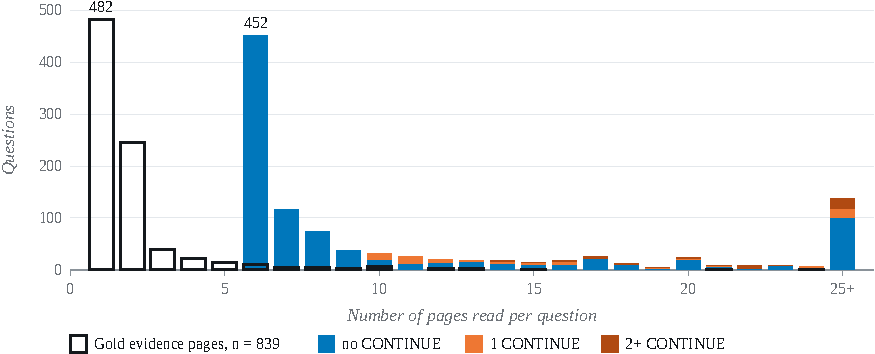
\includegraphics[width=0.9\columnwidth]{method/method_trajectory_v2.pdf}
    \caption{Trajectory of our method.}
    \label{fig:method_trajectory}
\end{figure}

\paragraph{Adaptive evidence acquisition.} Figure~\ref{fig:method_trajectory} shows that the pipeline does not uniformly consume its full page budget. The largest group terminates after six pages, the earliest point permitted by the stopping floor \(k=6\), while progressively fewer questions continue deeper into the retrieval ranking and a smaller group reaches the \(B=25\) limit. Reopened trajectories account for part of this longer tail, with some questions requiring one or multiple \texttt{CONTINUE} decisions after an initial synthesis attempt. This differs substantially from the annotated evidence distribution, where most answerable questions contain only one or two gold pages. The gap reflects the practical setting in which the locations of those pages are unknown and additional contextual pages may also contribute useful evidence.

% GENERATED by tables/scripts/method_cost.py -- do not edit by hand, re-run the script.
% Numbers read from results/method/telemetry_v5/per_turn_by_role.csv and per_question_summary.csv,
% written by `python -m seqread.build --iteration 5`.
\begin{table}[ht]
\centering
\small
\setlength{\tabcolsep}{5pt}
\renewcommand{\arraystretch}{1.12}
\adjustbox{max width=\textwidth}{%
\begin{tabular}{@{}l r rrr rr r@{}}
\toprule
& & \multicolumn{3}{c}{\textbf{Tokens}} & \multicolumn{2}{c}{\textbf{Latency (s)}} & \textbf{Peak} \\
\cmidrule(lr){3-5}\cmidrule(lr){6-7}
& \textbf{Turns} & \textbf{Input text} & \textbf{Input visual} & \textbf{Output} & \textbf{Prefill} & \textbf{Decode} & \textbf{VRAM (GiB)} \\
\midrule
\texttt{reader} & 11.2 & 5{,}209 & 834 & 1{,}008 & 2.0 & 70.6 & 7.3 \\
\texttt{synthesizer} & 1.4 & 9{,}638 & 1{,}742 & 724 & 4.0 & 59.0 & 8.2 \\
\texttt{arbiter} & 1.3 & 4{,}988 & 0 & 1{,}083 & 1.6 & 72.8 & 7.1 \\
\midrule
Per question, mean & 13.9 & 78{,}215 & 11{,}733 & 13{,}721 & 29.7 & 968.1 & 8.2 \\
Per question, median & 9.0 & 37{,}484 & 7{,}272 & 8{,}081 & 13.8 & 544.6 & 8.0 \\
\bottomrule
\end{tabular}%
}
\caption{Inference cost of the pipeline per agent turn and question.} % Over the 1{,}069 MMLongBench-Doc questions the pipeline finished, role rows give the mean per agent turn, with \textbf{Turns} the mean number of that role's turns per question; the per-question rows give each question's totals, with peak VRAM its highest turn. Every turn counts its completion passes. Visual tokens are those the language model receives after Qwen3-VL's patch merge. A question takes 16.6 minutes on average (median 9.4), almost all of it decoding, and no turn exceeds 13.4\,GiB.}
\label{tab:method_cost}
\end{table}

\paragraph{Inference cost.} Table~\ref{tab:method_cost} quantifies the cost of this adaptive behaviour. The pipeline uses 13.9 turns per question on average, compared with a median of 9.0, with the \texttt{reader} accounting for 11.2 turns and the \texttt{synthesizer} and \texttt{arbiter} invoked only 1.4 and 1.3 times per question respectively. Mean peak memory is 8.2\,GiB, remaining comfortably within the 16\,GB budget of the deployment GPU, while the average question consumes 78,215 text-input tokens, 11,733 visual tokens, and 13,721 output tokens across its trajectory. The principal cost is latency rather than memory: mean prefill time is only 29.7\,s per question compared with 968.1\,s of decoding, with a median total of roughly 9.3 minutes. The method therefore trades additional sequential inference for bounded memory use and broader evidence acquisition, with the deployment parameters providing a direct mechanism for reducing trajectory depth where lower latency is required.
